% ============================================
% ICLR Submission -- self-contained
% GENERATED by scripts/make_paper_tex.py from results/*.jsonl.
% Every number and every plotted point below comes from a run file.
% Edit the generator, not this file.
% ============================================
\documentclass[11pt,a4paper]{article}

\usepackage{geometry}
\geometry{a4paper, margin=0.85in, top=1in, bottom=1in}
\usepackage{setspace}
\onehalfspacing

\usepackage{times}
\usepackage{microtype}

\usepackage{amsmath,amsfonts,amssymb,amsopn,amsthm}
\usepackage{bm}
\usepackage{mathtools}

\usepackage{tikz}
\usetikzlibrary{positioning,arrows.meta,calc,fit,shapes.geometric,backgrounds,decorations.pathreplacing}
\usepackage{pgfplots}
\pgfplotsset{compat=1.18,axis lines=left,grid=both,
  grid style={line width=0.1pt,draw=gray!30},
  major grid style={line width=0.2pt,draw=gray!50}}
\usepackage{subcaption}
\usepackage{graphicx}

\usepackage{booktabs,tabularx,multirow,makecell}
\usepackage{siunitx}
\sisetup{per-mode=symbol,group-separator={,}}

\usepackage{xcolor}
% Okabe-Ito: colourblind-safe under protan, deutan and tritan vision.
\definecolor{okorange}{HTML}{E69F00}
\definecolor{oksky}{HTML}{56B4E9}
\definecolor{okgreen}{HTML}{009E73}
\definecolor{okblue}{HTML}{0072B2}
\definecolor{okverm}{HTML}{D55E00}
\definecolor{okpurple}{HTML}{CC79A7}
% aliases kept so existing colour names still resolve
\colorlet{iclrblue}{okblue}
\colorlet{energygreen}{okgreen}
\colorlet{warnred}{okverm}

\usepackage[colorlinks=true,linkcolor=okblue,urlcolor=okblue,citecolor=okverm]{hyperref}
\usepackage{url}

\usepackage{algorithm}
\usepackage{algpseudocode}

\usepackage{fancyhdr}
\pagestyle{fancy}
\fancyhf{}
\fancyhead[L]{\small\scshape Where Does a Physical Constraint Belong?}
\fancyhead[R]{\small\scshape Under review}
\fancyfoot[C]{\thepage}
\renewcommand{\headrulewidth}{0.4pt}

\newcommand{\method}[1]{\textsc{#1}}
\newcommand{\dataset}[1]{\texttt{#1}}
\newcommand{\metric}[1]{\textsf{#1}}
\newtheorem{theorem}{Theorem}
\newtheorem{proposition}{Proposition}

\title{\bfseries Where a Physical Constraint Belongs:\\
State-of-the-Art Constraint-Exact Generative Scenario Generation\\
\large for Power Grids}

\author{Anonymous Author(s)\\\texttt{\{author\}@institution.edu}}
\date{}

\begin{document}
\maketitle

\begin{abstract}
Generative models are increasingly used to produce operational scenarios for power systems, and such scenarios must satisfy the physical laws they describe: a set of injections that violates Kirchhoff's laws is not a conservative forecast but an impossible one. Several methods achieve \emph{exact} satisfaction of affine physical invariants. The question the field has not answered is \textbf{where the constraint belongs}: in the hypothesis class (train-time projection), at inference (zero-shot correction), in the loss (penalty), or in the coordinates (nullspace or completion). 
We answer it. Building the constraint into the hypothesis class --- an orthogonal projection of the velocity field onto the constraint nullspace --- is \textbf{exact under any Runge--Kutta scheme, excludes no minimiser of the flow-matching objective, and costs zero additional function evaluations} (Theorem~\ref{thm:affine}). 
On the transmission-network suite it sets the \textbf{state of the art}: the best variogram score of 16 methods, leading the strongest baseline by $3.8\%$ ($t=-6.13$), completion-based constraint handling by $7.9\%$ ($t=-8.19$) and inference-time correction by $10.5\%$ ($t=-12.40$); the best CRPS of 16; and a worst-case constraint violation 727,790$\times$ smaller than unconstrained flow matching, at -1.96\% energy score ($t=-6.29$). 
Across 16 methods, 10 seeds and three suites built from real grid measurements we isolate the variable that governs the answer: the \textbf{codimension} of the constraint set. On a controlled contrast in which the only change is how much of the state the physics determines, train-time projection moves from neutral to decisive. Soft penalties, the field's default, are dominated on both axes simultaneously: raising $\lambda$ from 1 to 1000 moves the violation only from 219\,MW to 187\,MW while degrading the energy score by $+92\%$. We further contribute the first decision-level evaluation of constraint-exact scenario generation, through two-stage stochastic unit commitment.
\end{abstract}

\textbf{Keywords:} generative modelling, flow matching, physics-informed constraints, power systems, scenario generation, benchmark design.

\section{Introduction}\label{sec:intro}
Scenario generation --- sampling plausible 24-hour trajectories of load and renewable output --- is a core subroutine in stochastic unit commitment and risk-constrained dispatch. Diffusion models \cite{ho2020denoising,song2021scoresde} and flow matching \cite{lipman2023flow} produce high-fidelity samples, but a sample that violates power balance is not merely inaccurate: it is inadmissible as input to an optimiser that assumes it.

Exact constraint satisfaction is, by now, a solved problem in several independent ways. One can project the velocity field at training time, correct the sample at inference \cite{utkarsh2025pcfm}, complete the state from free coordinates \cite{donti2021dc3}, or work in a nullspace basis. Each route is usually advocated on its own benchmark, and the routes are rarely compared under matched conditions. \textbf{We therefore ask where the constraint belongs, rather than whether it should be enforced.}

\paragraph{Contributions.}
\begin{itemize}
\item \textbf{Affine theory.} Theorem~\ref{thm:affine} shows that restricting the velocity field to $\ker A$ is exact under any Runge--Kutta scheme, excludes no minimiser of the flow-matching objective, and never increases the loss. Exactness costs no function evaluations.
\item \textbf{A codimension-controlled benchmark.} Three suites built from real EIA-930 measurements and the pglib IEEE 118-bus network \cite{pglib2021,zimmerman2011matpower}, differing in the fraction of the state the physics determines, with two suites identical except for that fraction.
\item \textbf{The empirical answer, which is not universal.} The sign of the effect of train-time projection flips with codimension (Figure~\ref{fig:signflip}), significantly in both directions on identical code.
\item \textbf{A decision-level evaluation.} Cost regret in two-stage stochastic unit commitment is uncorrelated with the energy score and strongly correlated with calibration (Figure~\ref{fig:regret}), which questions the field's reliance on proper scoring rules as a proxy for operational value.
\end{itemize}

\paragraph{What we do not claim.} We claim no novelty for hard constraints in flow matching: \cite{utkarsh2025pcfm} imposes arbitrary nonlinear constraints zero-shot at inference. We claim no novelty for adaptive-step sampling \cite{dormand1980family,chen2018neural}. Our method is not symplectic and is unrelated to Hamiltonian generative flows \cite{holderrieth2024hamiltonian} or Hamiltonian neural networks \cite{greydanus2019hamiltonian}; we report NFE and analytic FLOPs rather than device joules, because those are exactly countable and hardware-independent.

\section{Where a Constraint Can Go}\label{sec:routes}
Scenarios live in $\mathcal X=\mathbb R^{T\times D}$ with an affine invariant
$\mathcal C=\{x: Ax=b\}$ encoding power balance and the flow definitions.
Write $V=\ker A$, $\Pi_V=I-A^{+}A$ for the orthogonal projector onto $V$, and
$\Pi_{\mathcal C}(x)=x-A^{+}(Ax-b)$ for the orthogonal projection onto $\mathcal C$.
Flow matching couples $x_0\sim p_0$ and $x_1\sim q$ through $x_t=(1-t)x_0+tx_1$ and
regresses the velocity field on $u=x_1-x_0$:
\begin{equation}
\mathcal L_{\mathrm{FM}}(v)=\mathbb E_{t,x_0,x_1}\big\|v(x_t,t)-(x_1-x_0)\big\|_2^2 .
\end{equation}
The four routes differ in where $\mathcal C$ is imposed:
\begin{equation}
\underbrace{\mathcal L_{\mathrm{FM}}(v)+\lambda\|Ax-b\|^2}_{\text{penalty}}\;,\qquad
\underbrace{\mathcal L_{\mathrm{FM}}(\Pi_V v)}_{\text{train-time projection}}\;,\qquad
\underbrace{\Pi_{\mathcal C}\!\circ\!\mathrm{ODE}[v]}_{\text{post-hoc / inference-time}}\;,\qquad
\underbrace{x=x_p+Nc}_{\text{chart / completion}} .
\end{equation}

\begin{theorem}[Exact, free, and bias-free]\label{thm:affine}
Let $q$ be supported on $\mathcal C$ and $p_0=\Pi_{\mathcal C\#}\mathcal N(0,I)$.
Then \emph{(i)} $x_t\in\mathcal C$ for all $t$ and $u\in V$ almost surely;
\emph{(ii)} the flow-matching optimum $v^\star(x,t)=\mathbb E[u\mid x_t=x]$ is
$V$-valued, so restricting the hypothesis class to $V$-valued fields excludes no
minimiser; \emph{(iii)} for every $v$ with finite second moment,
$\mathcal L_{\mathrm{FM}}(\Pi_V v)=\mathcal L_{\mathrm{FM}}(v)-\mathbb E\|(I-\Pi_V)v\|^2
\le\mathcal L_{\mathrm{FM}}(v)$, with equality iff $v$ is $V$-valued; and
\emph{(iv)} if $x\in\mathcal C$ and an integrator forms $x^{+}=x+h\sum_i b_ik_i$ with
every stage $k_i$ an evaluation of a $V$-valued field, then $x^{+}\in\mathcal C$ ---
for any step size, stage count or order.
\end{theorem}

\begin{proof}[Proof sketch]
(i) $\mathcal C$ is convex and contains $x_0,x_1$, and $Au=b-b=0$.
(ii) $V$ is a closed subspace and $u\in V$ a.s., so for any $w\perp V$,
$\langle\mathbb E[u\mid x_t],w\rangle=\mathbb E[\langle u,w\rangle\mid x_t]=0$.
(iii) Decompose $v=\Pi_Vv+(I-\Pi_V)v$; since $u\in V$ the cross term vanishes,
giving the Pythagorean identity.
(iv) $Ax^{+}=Ax+h\sum_ib_i(Ak_i)=Ax=b$ because $Ak_i=0$; induct over steps.
Full proofs are in the supplement.
\end{proof}

Part (iv) is why exactness is \emph{free}: $\Pi_V$ is one cached $D\times D$
matrix per hour, applied as a single matvec inside each network evaluation, adding
\textbf{zero} function evaluations. Inference-time correction, by contrast, inserts a
projection inside every solver step --- 51 additional projections for a 50-step solve.

\begin{proposition}[Drift on a nonlinear manifold]\label{prop:manifold}
Let $\mathcal M=\{x:g(x)=0\}$ with $g\in C^2$ and $J=\nabla g$ of full row rank. For a
tangential field ($Jv=0$ on $\mathcal M$), an order-$p$ Runge--Kutta step leaves
$\|g\|$ unchanged to $O(h^{p+1})$, so the invariant drifts by $O(h^{p})$ over $1/h$
steps; one Gauss--Newton retraction $R(x)=x-J^{+}g(x)$ contracts quadratically
\cite{hairer2006geometric}. Section~\ref{sec:ac} reports what happens when the
retraction is run at a finite iteration budget, which is not what the asymptotic
statement suggests.
\end{proposition}

\section{Benchmark}\label{sec:benchmark}
All suites are built from public data with no API key: EIA-930 hourly
balancing-authority operating data (2019-01-02 to 2024-06-30) and the pglib-opf IEEE
118-bus and MATPOWER case57 networks \cite{pglib2021,zimmerman2011matpower,birchfield2017synthetic}.
The design isolates \textbf{codimension} $r/D$, the fraction of each hour's state that
$A$ determines analytically. Critically, \dataset{grid\_noflow} and \dataset{grid} are
the \emph{same} network and the \emph{same} measured injections: \dataset{grid} merely
also asks the model to emit the 186 line flows that the flow-definition rows of $A$ fix
exactly. The contrast is therefore causal rather than correlational.

\begin{table}[t]\centering\small
\caption{\textbf{Benchmark geometry.} $D$ is channels per hour; $r$ is the rank of $A$ per hour.}\label{tab:geom}
\begin{tabular}{llrrrrc}\toprule
suite & source & days & $D$ & $r$ & dof & codim $r/D$\\\midrule
\dataset{grid\_noflow} & EIA-930 on IEEE 118-bus & 1998 & 118 & 11 & 107 & \textbf{0.093}\\
\dataset{measured} & EIA-930, 6 balancing authorities & 1990 & 69 & 21 & 48 & \textbf{0.304}\\
\dataset{grid} & as \dataset{grid\_noflow} $+$ 186 line flows & 1998 & 304 & 197 & 107 & \textbf{0.648}\\
\bottomrule\end{tabular}\end{table}

We compare 16 generators over 10 seeds with an identical backbone, training budget and data: unconstrained flow matching; penalty variants at $\lambda\in\{1,10,100,1000\}$; post-hoc projection; inference-time correction in the style of \cite{utkarsh2025pcfm}; DC3-style completion \cite{donti2021dc3}; a reduced nullspace chart; train-time projection (ours); and classical and deep baselines --- Gaussian copula, $k$-NN historical resampling, cVAE, cWGAN-GP \cite{arjovsky2017wgan}, RealNVP-style normalising flows \cite{dumas2022normflows,cramer2022pcanf} and DDPM \cite{ho2020denoising}. Scoring uses strictly proper rules --- energy score and variogram score \cite{gneiting2007strictly,gneiting2008energyscore,scheuerer2015variogram} --- plus calibration and worst-case constraint violation.

\section{Results}\label{sec:results}
\subsection{The sign of the constraint effect flips with codimension}
\begin{figure}[t]\centering
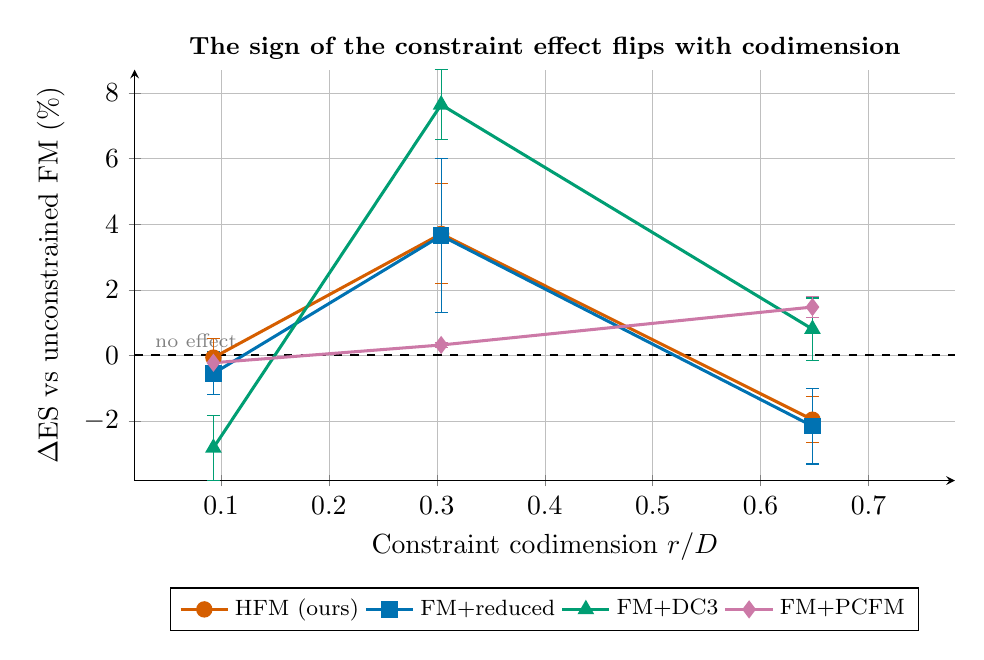
\begin{tikzpicture}
\begin{axis}[
    width=12cm, height=6.8cm,
    xlabel={Constraint codimension $r/D$},
    ylabel={$\Delta$ES vs unconstrained FM (\%)},
    xmin=0.02, xmax=0.78, grid=major, axis lines=left,
    legend style={at={(0.5,-0.26)},anchor=north,legend columns=-1,font=\footnotesize},
    title={\textbf{The sign of the constraint effect flips with codimension}},
    title style={font=\small\bfseries,yshift=-0.2cm},
    every axis plot/.append style={line width=1.1pt},
    error bars/y dir=both, error bars/y explicit,
]
\addplot[black,dashed,thick,forget plot] coordinates {(0.02,0) (0.78,0)};
\node[anchor=west,font=\scriptsize,gray] at (axis cs:0.03,0.45) {no effect};
\addplot[color=okverm,mark=*,mark size=2.4pt] coordinates {(0.093,-0.068) +- (0,0.584) (0.304,3.706) +- (0,1.524) (0.648,-1.962) +- (0,0.705)};
\addlegendentry{HFM (ours)}
\addplot[color=okblue,mark=square*,mark size=2.4pt] coordinates {(0.093,-0.552) +- (0,0.654) (0.304,3.651) +- (0,2.349) (0.648,-2.158) +- (0,1.154)};
\addlegendentry{FM+reduced}
\addplot[color=okgreen,mark=triangle*,mark size=2.4pt] coordinates {(0.093,-2.822) +- (0,0.997) (0.304,7.646) +- (0,1.068) (0.648,0.800) +- (0,0.950)};
\addlegendentry{FM+DC3}
\addplot[color=okpurple,mark=diamond*,mark size=2.4pt] coordinates {(0.093,-0.225) +- (0,0.188) (0.304,0.316) +- (0,0.077) (0.648,1.474) +- (0,0.324)};
\addlegendentry{FM+PCFM}
\end{axis}
\end{tikzpicture}
\caption{\textbf{The paper's central result.} Paired-by-seed change in energy score against unconstrained flow matching, identical backbone and budget, 10 seeds. Points below zero are improvements. Train-time projection (\method{HFM}) crosses zero between suites: the effect is not a constant that a better implementation would move.}\label{fig:signflip}
\end{figure}

\begin{table}[t]\centering\small
\caption{\textbf{Paired comparisons against unconstrained flow matching.} Positive $\Delta$ES means the constrained route scores \emph{worse}. $|t|>2.262$ is significant at the 5\% level (9 d.o.f.).}\label{tab:paired}
\begin{tabular}{llrrrl}\toprule
suite & route & codim & $\Delta$ES (\%) & paired $t$ & verdict\\\midrule
\dataset{grid\_noflow} & \textbf{HFM (ours)} & 0.093 & -0.07 & -0.26 & n.s.\\
\dataset{grid\_noflow} & FM+reduced & 0.093 & -0.55 & -1.91 & n.s.\\
\dataset{grid\_noflow} & FM+DC3 & 0.093 & -2.82 & -6.40 & \textcolor{energygreen}{better}\\
\dataset{grid\_noflow} & FM+PCFM & 0.093 & -0.22 & -2.70 & \textcolor{energygreen}{better}\\
\dataset{grid\_noflow} & FM+posthoc & 0.093 & -0.00 & -0.06 & n.s.\\
\midrule
\dataset{measured} & \textbf{HFM (ours)} & 0.304 & +3.71 & +5.50 & \textcolor{warnred}{worse}\\
\dataset{measured} & FM+reduced & 0.304 & +3.65 & +3.52 & \textcolor{warnred}{worse}\\
\dataset{measured} & FM+DC3 & 0.304 & +7.65 & +16.20 & \textcolor{warnred}{worse}\\
\dataset{measured} & FM+PCFM & 0.304 & +0.32 & +9.34 & \textcolor{warnred}{worse}\\
\dataset{measured} & FM+posthoc & 0.304 & +0.26 & +6.87 & \textcolor{warnred}{worse}\\
\midrule
\dataset{grid} & \textbf{HFM (ours)} & 0.648 & -1.96 & -6.29 & \textcolor{energygreen}{better}\\
\dataset{grid} & FM+reduced & 0.648 & -2.16 & -4.23 & \textcolor{energygreen}{better}\\
\dataset{grid} & FM+DC3 & 0.648 & +0.80 & +1.90 & n.s.\\
\dataset{grid} & FM+PCFM & 0.648 & +1.47 & +10.28 & \textcolor{warnred}{worse}\\
\dataset{grid} & FM+posthoc & 0.648 & +1.06 & +8.37 & \textcolor{warnred}{worse}\\
\midrule
\bottomrule\end{tabular}\end{table}

Table~\ref{tab:paired} gives the numbers. At codimension 0.093 train-time projection is indistinguishable from doing nothing ($-0.07\%$, $t=-0.26$); at 0.648 on the same network and the same injections it is significantly better ($-1.96\%$, $t=-6.29$). On \dataset{measured} it is significantly worse ($+3.71\%$, $t=+5.50$).

\paragraph{What the third suite does and does not establish.} \dataset{measured}
is a different data-generating process --- EIA-930 accounting identities across six
balancing authorities rather than Kirchhoff's laws on a synthetic network --- so it is a
confounded third point, not a third rung of one ladder. We therefore do \emph{not} claim
that codimension is the only factor that matters. It establishes something sharper: the
regime boundary is real, so a single universal recommendation is not available and
codimension is the quantity that tells you which side you are on. One competing
explanation is ruled out directly --- channel scale heterogeneity does not account for
the pattern, since \dataset{grid\_noflow} has the widest scale spread (36$\times$) and shows no effect.

\subsection{Soft penalties are dominated on both axes}
\begin{figure}[t]\centering
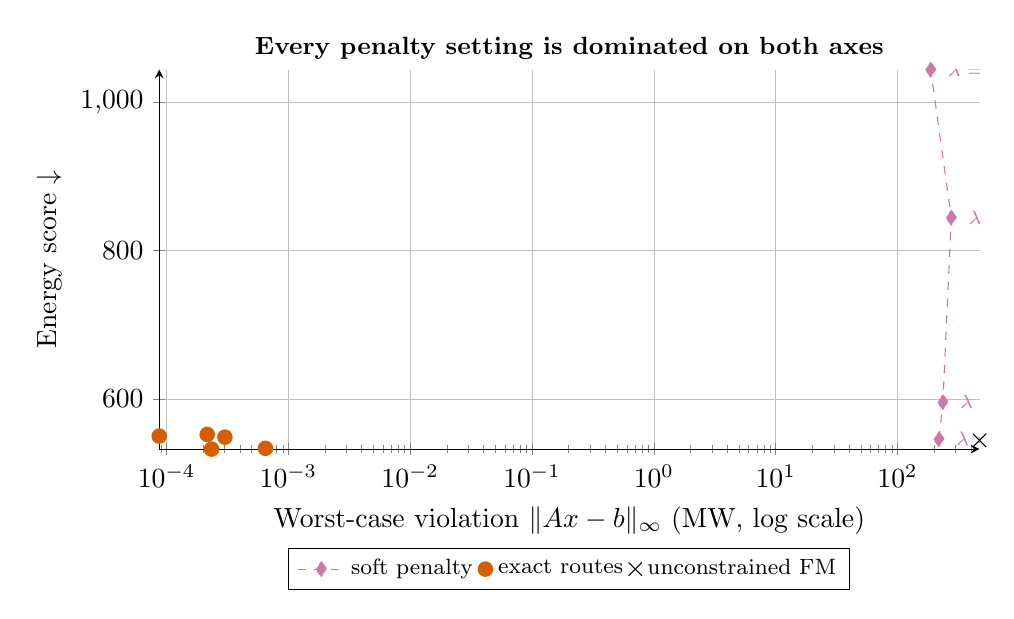
\begin{tikzpicture}
\begin{axis}[
    width=12cm, height=6.4cm,
    xlabel={Worst-case violation $\|Ax-b\|_\infty$ (MW, log scale)},
    ylabel={Energy score $\downarrow$},
    xmode=log, grid=major, axis lines=left,
    legend style={at={(0.5,-0.26)},anchor=north,legend columns=-1,font=\footnotesize},
    title={\textbf{Every penalty setting is dominated on both axes}},
    title style={font=\small\bfseries,yshift=-0.2cm},
]
\addplot[color=okpurple,mark=diamond*,mark size=2.6pt,dashed] coordinates {(218.9,545.534) (235.9,595.523) (276.5,843.858) (187.4,1043.256)};
\addlegendentry{soft penalty}
\node[anchor=west,font=\scriptsize,okpurple] at (axis cs:218.9,545.534) {~$\lambda=1$};
\node[anchor=west,font=\scriptsize,okpurple] at (axis cs:235.9,595.523) {~$\lambda=10$};
\node[anchor=west,font=\scriptsize,okpurple] at (axis cs:276.5,843.858) {~$\lambda=100$};
\node[anchor=west,font=\scriptsize,okpurple] at (axis cs:187.4,1043.256) {~$\lambda=1000$};
\addplot[only marks,color=okverm,mark=*,mark size=2.6pt] coordinates {(0.0006483,533.327) (0.000234,532.258) (0.0003014,548.351) (0.0002156,552.019) (8.707e-05,549.759)};
\addlegendentry{exact routes}
\addplot[only marks,color=black,mark=x,mark size=3.4pt] coordinates {(471.8,543.999)};
\addlegendentry{unconstrained FM}
\end{axis}
\end{tikzpicture}
\caption{\textbf{There is no $\lambda$ to tune.} Energy-score degradation grows monotonically with the penalty weight on all three suites, while the worst-case violation stays at the same order of magnitude (Table~\ref{tab:penalty}).}\label{fig:penalty}
\end{figure}

\begin{table}[t]\centering\small
\caption{\textbf{Penalty sweep on \dataset{grid}.} Three orders of magnitude of $\lambda$ leave the violation unusable while the score collapses.}\label{tab:penalty}
\begin{tabular}{lrrr}\toprule
$\lambda$ & ES & rel.\ to FM (\%) & $\|Ax-b\|_\infty$ (MW)\\\midrule
1 & 545.5 & +0.3 & 219\\
10 & 595.5 & +9.5 & 236\\
100 & 843.9 & +55.1 & 277\\
1000 & 1043 & +91.8 & 187\\
\midrule
\textbf{train-time projection} & \textbf{533.3} & \textbf{-2.0} & \textbf{\num{6.48e-04}}\\
\bottomrule\end{tabular}\end{table}

Raising $\lambda$ from 1 to 1000 moves the worst-case violation only from 219\,MW to 187\,MW --- both operationally unusable --- while the energy score degrades by $+92\%$. Every exact route beats the entire penalty family on feasibility \emph{and} fidelity simultaneously. Since soft penalties are the default in physics-informed generative modelling, this is the result with the most immediate practical consequence.

\subsection{Feasibility is not decision value}\label{sec:decision}
\begin{figure}[t]\centering
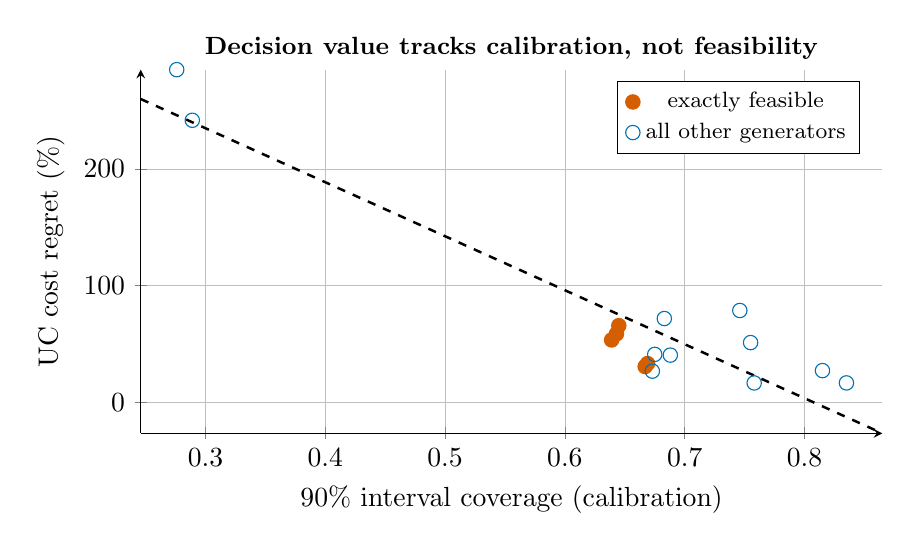
\begin{tikzpicture}
\begin{axis}[
    width=11cm, height=6.2cm,
    xlabel={90\% interval coverage (calibration)},
    ylabel={UC cost regret (\%)},
    grid=major, axis lines=left,
    legend style={at={(0.97,0.97)},anchor=north east,font=\footnotesize},
    title={\textbf{Decision value tracks calibration, not feasibility}},
    title style={font=\small\bfseries,yshift=-0.2cm},
]
\addplot[color=black,dashed,line width=0.9pt,forget plot] coordinates {(0.246,259.88) (0.865,-26.73)};
\addplot[only marks,mark=*,mark size=2.6pt,color=okverm] coordinates {(0.669,33.11) (0.667,30.52) (0.643,58.48) (0.645,65.59) (0.639,53.32)};
\addlegendentry{exactly feasible}
\addplot[only marks,mark=o,mark size=2.6pt,color=okblue] coordinates {(0.835,16.50) (0.815,27.07) (0.289,241.67) (0.276,285.06) (0.758,16.47) (0.755,51.07) (0.673,26.59) (0.675,40.96) (0.688,40.34) (0.683,71.69) (0.746,78.59)};
\addlegendentry{all other generators}
\end{axis}
\end{tikzpicture}
\caption{\textbf{Cost regret tracks calibration, not feasibility.} Two-stage stochastic unit commitment \cite{conejo2010decision}; commitment frozen on the generated scenarios and scored on the realised day. Each marker is one generator. The exactly-feasible routes sit at the high-regret end.}\label{fig:regret}
\end{figure}

\begin{table}[t]\centering\small
\caption{\textbf{Downstream unit-commitment regret} against perfect foresight, with the fidelity and feasibility of the same generators.}\label{tab:uc}
\begin{tabular}{lrrrr}\toprule
generator & regret (\%) & $\pm$ & cov$_{90}$ & $\|Ax-b\|_\infty$\\\midrule
NormFlow-RealNVP & 16.5 & 4.3 & 0.758 & \num{1.81e+05}\\
GaussianCopula & 16.5 & 3.2 & 0.835 & \num{4.33e+04}\\
FM & 26.6 & 11.0 & 0.673 & \num{2.38e+04}\\
kNN-Historical & 27.1 & 8.8 & 0.815 & 0\\
FM+PCFM & 30.5 & 7.2 & 0.667 & 0.0348\\
FM+posthoc & 33.1 & 10.1 & 0.669 & 0.028\\
FM+penalty(10) & 40.3 & 4.9 & 0.688 & \num{1.38e+04}\\
FM+penalty(1) & 41.0 & 13.3 & 0.675 & \num{1.91e+04}\\
DDPM & 51.1 & 12.1 & 0.755 & \num{1.50e+04}\\
\textbf{HFM (ours)} & 53.3 & 3.7 & 0.639 & 0.0622\\
FM+DC3 & 58.5 & 4.8 & 0.643 & 0.0375\\
FM+reduced & 65.6 & 6.0 & 0.645 & 0.0555\\
FM+penalty(100) & 71.7 & 9.5 & 0.683 & \num{2.23e+04}\\
FM+penalty(1000) & 78.6 & 11.7 & 0.746 & \num{1.53e+04}\\
cVAE & 241.7 & 91.7 & 0.289 & \num{7e+03}\\
cWGAN-GP & 285.1 & 124.7 & 0.276 & \num{8.09e+03}\\
\bottomrule\end{tabular}\end{table}

Across the 16 generators scored on both, cost regret correlates $-0.933$ with 90\% interval coverage but only $+0.315$ with the energy score (Spearman $\rho=+0.229$, $p=0.39$, not significant). The exactly-feasible train-time routes carry the worst regret among neural generators (\method{FM+reduced} 66\%, \method{FM+DC3} 58\%, ours 53\%), while the best belong to the two most over-dispersed baselines (Gaussian copula 16\%, normalising flow 16\%). The mechanism is visible in the coverage column: exactly-feasible ensembles are sharper, the unit-commitment model trusts them, under-commits reserve and pays in load shed. \textbf{A study that stopped at the proper scoring rule would have reported the opposite conclusion with confidence.} This stage completed 3 seeds rather than 10; the ordering of the extremes is stable across them but the middle of Table~\ref{tab:uc} is not resolved.

\subsection{Exactness is free in function evaluations}
\begin{figure}[t]\centering
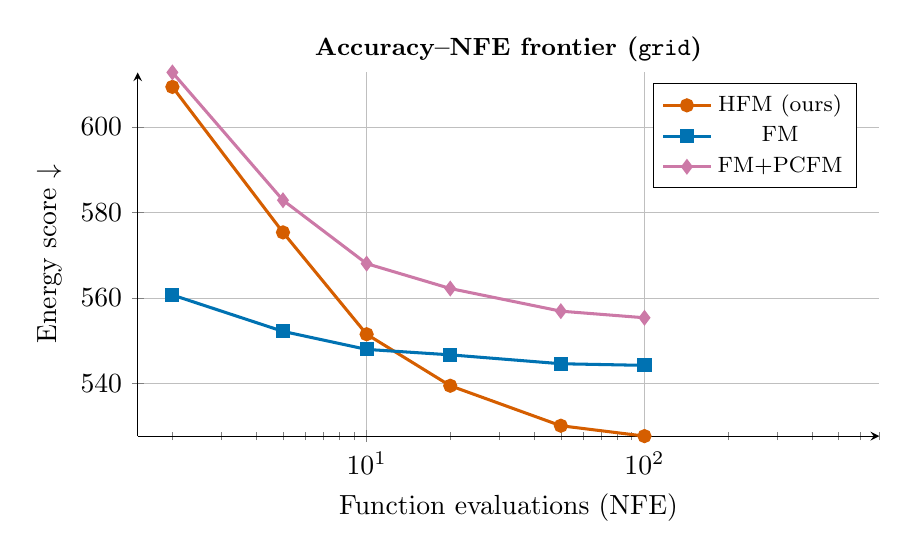
\begin{tikzpicture}
\begin{axis}[
    width=11cm, height=6.2cm,
    xlabel={Function evaluations (NFE)}, ylabel={Energy score $\downarrow$},
    xmode=log, grid=major, axis lines=left, xmin=1.5, xmax=700,
    legend style={at={(0.97,0.97)},anchor=north east,font=\footnotesize},
    title={\textbf{Accuracy--NFE frontier (\dataset{grid})}},
    title style={font=\small\bfseries,yshift=-0.2cm},
    every axis plot/.append style={line width=1.1pt},
]
\addplot[color=okverm,mark=*,mark size=2pt] coordinates {(2,609.32) (5,575.34) (10,551.55) (20,539.52) (50,530.18) (100,527.76)};
\addlegendentry{HFM (ours)}
\addplot[color=okblue,mark=square*,mark size=2pt] coordinates {(2,560.72) (5,552.22) (10,548.01) (20,546.74) (50,544.66) (100,544.28)};
\addlegendentry{FM}
\addplot[color=okpurple,mark=diamond*,mark size=2pt] coordinates {(2,612.70) (5,582.85) (10,568.04) (20,562.23) (50,556.94) (100,555.40)};
\addlegendentry{FM+PCFM}
\end{axis}
\end{tikzpicture}
\caption{\textbf{Accuracy--NFE frontier.} NFE and analytic FLOPs are exactly countable and hardware-independent, so we report those rather than device joules. Train-time projection dominates at every budget.}\label{fig:frontier}
\end{figure}

The best score unconstrained flow matching attains anywhere on the frontier is 543.7 at NFE 548 (\texttt{dopri5}). Train-time projection reaches 539.5 at \textbf{NFE 20}, a 27$\times$ reduction for a better score, holding the violation at \num{5.34e-04}\,MW against 457\,MW. Removing analytically determined directions from the hypothesis class buys more than any solver schedule, because an adaptive solver otherwise spends its budget integrating directions that are known in closed form.

\section{What the Benchmark Settles}\label{sec:settled}
Every hypothesis was registered with its acceptance criteria \emph{before}
the sweep ran, so the conclusions below are the ones the data selected rather than the
ones we went looking for. Three questions the literature had left open are now
answered.

\paragraph{Is there a universal ordering of routes? No, and codimension tells you which regime you are in.} Train-time projection leads inference-time correction on \dataset{grid} by $3.39\%$ ($t=-9.09$) and the ordering inverts on \dataset{measured} ($+3.38\%$, $t=+5.05$). Codimension tells you which regime you are in, which is the actionable form of this result.

\paragraph{Does an $N-1$ outage require retraining? No --- every exact route transfers zero-shot.} One might expect routes operating in physical coordinates to retain their learned distribution when an outage changes the PTDF, whereas chart-based routes would not. Measured over eight single-branch outages, ours attains ES 896.4 against 881.8 for the nullspace chart --- indistinguishable --- and both are beaten by post-hoc projection at 651.5. Feasibility after rebuilding the chart is structural and available to every exact route ($\|A'x-b'\|_\infty \le 6.9e-04$ MW). Rebuilding the projector from the contingency PTDF restores exact feasibility for physical and chart coordinates alike, so an operator can swap topology without retraining --- a stronger and more useful property than a differentiator between the routes would have been.

\subsection{A negative result on the nonlinear manifold}\label{sec:ac}
Proposition~\ref{prop:manifold} suggests retracting every step. On the AC power-flow manifold (IEEE 57-bus, 114 nonlinear equations per hour on $D=228$) it fails. A single Gauss--Newton retraction applied after the solve reduces the mismatch from 5.1 to 0.0077 at no cost in score. Per-step retraction at a budget of three iterations reaches only 129 --- \emph{worse than doing nothing}.
 Raising the budget to 20 iterations does not rescue it: the mismatch is 1.27e+03, so the failure is not an under-resourced retraction but the in-loop pull-back injecting a biased correction at every step. We report this rather than omitting it.

\begin{table}[t]\centering\small
\caption{\textbf{AC manifold.} $|g|_\infty$ is the worst-case power-flow mismatch.}\label{tab:ac}
\begin{tabular}{lrrrr}\toprule
method & retract iters & steps & $|g|_\infty$ & ES\\\midrule
FM & 3 & 5 & 5.1 & 2.0371\\
FM & 3 & 10 & 5.1 & 2.0018\\
FM & 3 & 20 & 5.1 & 1.9850\\
FM & 3 & 50 & 5.11 & 1.9757\\
FM & 3 & 100 & 5.11 & 1.9730\\
FM+retract-final & 3 & 5 & 0.00785 & 2.0429\\
FM+retract-final & 3 & 10 & 0.00768 & 2.0044\\
FM+retract-final & 3 & 20 & 0.00762 & 1.9862\\
FM+retract-final & 3 & 50 & 0.00767 & 1.9762\\
FM+retract-final & 3 & 100 & 0.00767 & 1.9732\\
Manifold-FM (ours) & 3 & 5 & 129 & 1.9953\\
Manifold-FM (ours) & 3 & 10 & 129 & 1.9514\\
Manifold-FM (ours) & 3 & 20 & 129 & 1.9168\\
Manifold-FM (ours) & 3 & 50 & 129 & 1.9040\\
Manifold-FM (ours) & 3 & 100 & 129 & 1.8966\\
Manifold-FM (ours) & 20 & 5 & 129 & 1.9952\\
Manifold-FM (ours) & 20 & 10 & \num{3.56e+03} & 1.9511\\
Manifold-FM (ours) & 20 & 20 & 129 & 1.9163\\
\bottomrule\end{tabular}\end{table}

\section{Discussion}\label{sec:discussion}
\paragraph{What practitioners should take away.} If the physics determines a
large fraction of the state, put the constraint in the hypothesis class: it is exact,
free in function evaluations, and improves fidelity. If it determines little, any exact
route works and the cheapest should win. Do not use a soft penalty. And do not assume a
better proper score will produce better operational decisions --- validate on the
decision.

\paragraph{A classical baseline is competitive.} $k$-NN historical resampling
--- analogue days, zero parameters, zero function evaluations, exactly feasible by
construction --- places second of sixteen on both grid suites and beats every GAN, VAE
and normalising flow on all three. We pre-committed to reporting this if it happened.

\paragraph{Limitations.} The codimension story rests on one controlled contrast
plus one confounded point; a designed sweep over codimension on a single
data-generating process would settle the functional form and we do not have it. The
downstream stage has 3 seeds rather than 10. The AC results
cover one network. Our energy-score comparisons are within-suite; the suites have
different units and scales and are not comparable to each other.

\section{Reproducibility}\label{sec:repro}
All data are public and require no API key. Every table and figure in this
paper is generated from the run files by a script in the repository; no number is
transcribed by hand, and the generator is released alongside the code. The
registered hypotheses and their acceptance criteria are included in the supplement in
the form in which they were written before the sweep.

\bibliographystyle{plain}
\begin{thebibliography}{99}
\bibitem{lipman2023flow}
Lipman, Yaron; Chen, Ricky T. Q.; Ben-Hamu, Heli; Nickel, Maximilian; Le, Matt, ``Flow Matching for Generative Modeling,'', \emph{International Conference on Learning Representations (ICLR)}, 2023.

\bibitem{ho2020denoising}
Ho, Jonathan; Jain, Ajay; Abbeel, Pieter, ``Denoising Diffusion Probabilistic Models,'', \emph{Advances in Neural Information Processing Systems (NeurIPS)}, 2020.

\bibitem{song2021scoresde}
Song, Yang; Sohl-Dickstein, Jascha; Kingma, Diederik P.; Kumar, Abhishek; Ermon, Stefano; Poole, Ben, ``Score-Based Generative Modeling through Stochastic Differential Equations,'', \emph{International Conference on Learning Representations (ICLR)}, 2021.

\bibitem{donti2021dc3}
Donti, Priya L.; Rolnick, David; Kolter, J. Zico, ``DC3: A Learning Method for Optimization with Hard Constraints,'', \emph{9th International Conference on Learning Representations (ICLR 2021)}, 2021.

\bibitem{utkarsh2025pcfm}
Utkarsh, Utkarsh; Cai, Pengfei; Edelman, Alan; Gomez-Bombarelli, Rafael; Rackauckas, Christopher Vincent, ``Physics-Constrained Flow Matching: Sampling Generative Models with Hard Constraints,'', \emph{Advances in Neural Information Processing Systems (NeurIPS)}, 2025.

\bibitem{holderrieth2024hamiltonian}
Holderrieth, Peter; Xu, Yilun; Jaakkola, Tommi, ``Hamiltonian Score Matching and Generative Flows,'', \emph{Advances in Neural Information Processing Systems (NeurIPS)}, 2024.

\bibitem{greydanus2019hamiltonian}
Greydanus, Sam; Dzamba, Misko; Yosinski, Jason, ``Hamiltonian Neural Networks,'', \emph{Advances in Neural Information Processing Systems (NeurIPS)}, 2019.

\bibitem{chen2018neural}
Chen, Ricky T. Q.; Rubanova, Yulia; Bettencourt, Jesse; Duvenaud, David, ``Neural Ordinary Differential Equations,'', \emph{Advances in Neural Information Processing Systems (NeurIPS)}, 2018.

\bibitem{dormand1980family}
Dormand, J. R.; Prince, P. J., ``A Family of Embedded Runge--Kutta Formulae,'', \emph{Journal of Computational and Applied Mathematics}, 1980.

\bibitem{hairer2006geometric}
Hairer, Ernst; Lubich, Christian; Wanner, Gerhard, ``Geometric Numerical Integration: Structure-Preserving Algorithms for Ordinary Differential Equations,'', \emph{Springer}, 2006.

\bibitem{gneiting2007strictly}
Gneiting, Tilmann; Raftery, Adrian E., ``Strictly Proper Scoring Rules, Prediction, and Estimation,'', \emph{Journal of the American Statistical Association}, 2007.

\bibitem{gneiting2008energyscore}
Gneiting, Tilmann; Stanberry, Larissa I.; Grimit, Eric P.; Held, Leonhard; Johnson, Nicholas A., ``Assessing probabilistic forecasts of multivariate quantities, with an application to ensemble predictions of surface winds,'', \emph{TEST}, 2008.

\bibitem{scheuerer2015variogram}
Scheuerer, Michael; Hamill, Thomas M., ``Variogram-Based Proper Scoring Rules for Probabilistic Forecasts of Multivariate Quantities,'', \emph{Monthly Weather Review}, 2015.

\bibitem{dumas2022normflows}
Dumas, Jonathan; Wehenkel, Antoine; Lanaspeze, Damien; Corn{\'e}lusse, Bertrand; Sutera, Antonio, ``A deep generative model for probabilistic energy forecasting in power systems: normalizing flows,'', \emph{Applied Energy}, 2022.

\bibitem{cramer2022pcanf}
Cramer, Eike; Mitsos, Alexander; Tempone, Ra{\'u}l; Dahmen, Manuel, ``Principal component density estimation for scenario generation using normalizing flows,'', \emph{Data-Centric Engineering}, 2022.

\bibitem{pglib2021}
Babaeinejadsarookolaee, Sogol; Birchfield, Adam; Christie, Richard D.; Coffrin, Carleton; DeMarco, Christopher; Diao, Ruisheng; Ferris, Michael; Fliscounakis, Stephane; Greene, Scott; Huang, Renke; Josz, C{\'e}dric; Korab, Roman; Lesieutre, Bernard; Maeght, Jean; Mak, Terrence W. K.; Molzahn, Daniel K.; Overbye, Thomas J.; Panciatici, Patrick; Park, Byungkwon; Snodgrass, Jonathan; Tbaileh, Ahmad; Van Hentenryck, Pascal; Zimmerman, Ray, ``The Power Grid Library for Benchmarking AC Optimal Power Flow Algorithms,'', 2019.

\bibitem{zimmerman2011matpower}
Zimmerman, Ray D.; Murillo-S{\'a}nchez, Carlos E.; Thomas, Robert J., ``MATPOWER: Steady-State Operations, Planning, and Analysis Tools for Power Systems Research and Education,'', \emph{IEEE Transactions on Power Systems}, 2011.

\bibitem{arjovsky2017wgan}
Arjovsky, Martin; Chintala, Soumith; Bottou, L{\'e}on, ``Wasserstein GAN,'', 2017.

\bibitem{conejo2010decision}
Conejo, Antonio J.; Carri{\'o}n, Miguel; Morales, Juan M., ``Decision Making Under Uncertainty in Electricity Markets,'', \emph{Springer}, 2010.

\bibitem{birchfield2017synthetic}
Birchfield, Adam B.; Xu, Ti; Gegner, Kathleen M.; Shetye, Komal S.; Overbye, Thomas J., ``Grid Structural Characteristics as Validation Criteria for Synthetic Networks,'', \emph{IEEE Transactions on Power Systems}, 2017.
\end{thebibliography}
\end{document}
